\begin{section}{Results}
  \label{sec:results}
  We now present the results of a simulation of $128^3$ neutrinos 
with mass 0.2eV and $64^3$ dark matter particles. The simulation 
is done in a box of size $500 Mpc/h$. As noted above, initial 
conditions for dark matter particles are produced at $z=100$ 
whereas neutrinos are introduced at $z=10$. We take cosmological 
parameters which are in line with the most recent Planck results 
\cite{bib:Planck2015}: $h=0.67,\, \Omega_b=0.05, \Omega_c=0.27, 
\sigma_8=0.83,\, n_s=0.96 $, and

\begin{equation}
  \Omega_\nu = \frac{m_\nu}{93.14 h^2}
\end{equation}
We assume a flat universe and so set $\Omega_\Lambda=1-\Omega_m=1-\Omega_b-\Omega_c-\Omega_\nu$.

\par The dimensionless density power spectra of the four velocity 
bins are depicted in Fig. \ref{fig:denpowerfig}. We find that 
neutrinos with smaller initial velocities have greater power at all scales 
with the difference in power between the velocity bins increasing at smaller scales. 
This is to be expected as less energetic neutrinos are more easily trapped 
in potential wells and thus tend to cluster, resulting in an overdensity at all -
but particularly small - scales relative to more energetic neutrinos. 
This also results in the power spectra of the neutrinos with the 
smallest initial velocities deviating the most from linear theory predictions. 
The velocity power spectra are shown in Fig. \ref{fig:velpowerfig}.
A similar pattern is evident as neutrinos with smaller initial velocity have
greater power at all scales. The velocities of less energetic neutrinos are
more likely to be correlated (particularly over small scales) as they will
more easily be focused into clusters with a coherent velocity than neutrinos
with large initial velocities. 

\begin{figure}[htbp]
  \begin{center}
    \includegraphics[width=0.5\textwidth]{./figures/DensityPowerSpectra/denpower.pdf}
    \caption{(Placeholder) Density power spectra of the four neutrino velocity bins
	      at z=0 (solid lines). Also plotted are the power spectra predicted by
	      linear theory (dashed lines).}
    \label{fig:denpowerfig}
  \end{center}
\end{figure}

\begin{figure}[htbp]
  \begin{center}
    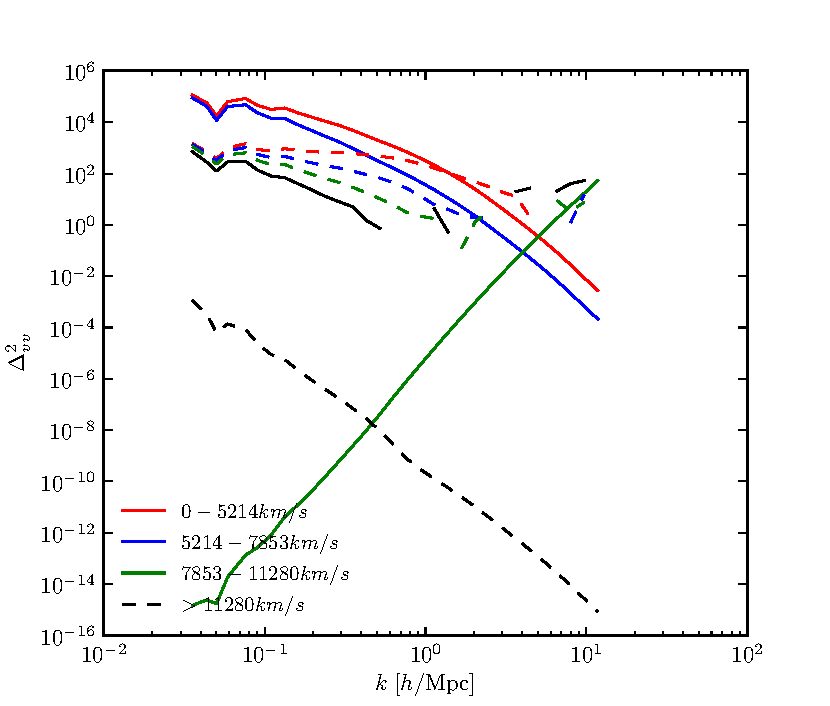
\includegraphics[width=0.5\textwidth]{./figures/VelPowerSpectra/velpower.pdf}
    \caption{(Placeholder) Velocity power spectra of the four neutrino velocity
	      bins at z=0 (dashed lines) compared with the reconstructed velocity
	      power spectra (solid lines).}
    \label{fig:velpowerfig}
  \end{center}
\end{figure}

\par Lastly, Fig. \ref{fig:dipolefig} depicts the dipole correlation 
functions for each velocity bin calculated using the neutrino
velocity field produced from the momentum method and the velocity 
field reconstructed from the CDM and halo density fields. For $r>5\mpch$ 
there is little difference between most of the dipole correlation functions
calculated using the different methods and the velocity bins. However the
dipole corresponding to the $0-5214km/s$ bin with the CDM 
reconstruction method is markedly smaller than those of the other bins. 
For smaller $r$, the dipoles for the larger velocity bins begin to
dominate the smaller velocity bins; this is particularly pronounced in 
the dipole functions produced using the CDM reconstructed velocity fields.

\begin{figure}[htbp]
  \begin{center}
    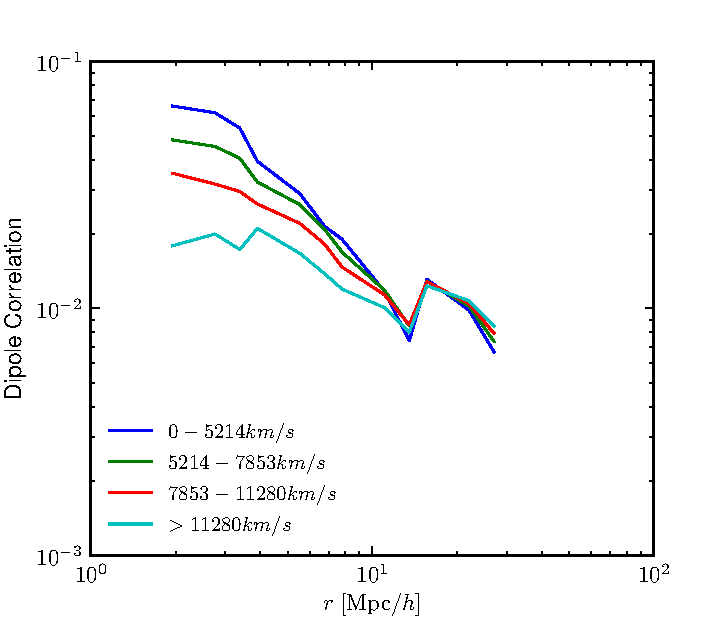
\includegraphics[width=0.5\textwidth]{./figures/Dipole/dipolefig.pdf}
    \caption{(Placeholder) Dipole correlation functions for each neutrino
	      velocity bin at z=0 calculated using the momentum method
	      velocity field (solid lines), reconstruction using the CDM 
	      density field (dashed lines), and reconstruction using the halo
	      density field (dot-dash lines).}
    \label{fig:dipolefig}
  \end{center}
\end{figure}

\end{section}
